\algorithm{Boolean Variable Splitting}%
          {A. Huntwork and X. Zhang}


\section{Introduction}
This algorithm detects boolean variables and arrays and modifies 
all uses and definitions of these variables.  In particular, every 
variable or array element is split into 2 variables or array elements,
and the state of the original variable is reflected in the combined 
state of these 2 variables or array elements. 
This algorithm consists of two components. One is 
 boolean variable identification. We implement a dataflow analysis algorithm over the
control flow graph which can identify the range of possible values of any variable.
From the range the variable we can tell if it is a boolean variable
(range between 0 and 1). The other is splitting the variables 
that are recognized. We implement 3 splitting algorithms, described below.

\section{Boolean variable recognition}

\subsection{Observations}

\begin{itemize}
\item Boolean variables in method fields have Z type
\item Boolean variables in method parameters have Z type
\item Boolean functions have Z return type
\item Boolean local variables have implicit I type (which means iload is used
to load the variable, istore is used to store)
\item An assignment to a boolean variable in java source code generates
the following java bytecode sequence:
\end{itemize}
\emph{~~~~~ifeq l1}

\emph{~~~~~iconst\_0}

\emph{~~~~~goto l2}

\emph{~~~~~l1:}

\emph{~~~~~iconst\_1}

\emph{~~~~~l2:}

\emph{~~~~~istore boolean\_var}

\begin{itemize}
\item An boolean operation is implemented similarly. For example,
b=a\&\&c generates the following code sequence:
\end{itemize}
\emph{~~~~iload a }

\emph{~~~~ifeq l1}

\emph{~~~~iload c }

\emph{~~~~ifeq l1 }

\emph{~~~~iconst\_1 }

\emph{~~~~goto l2 }

\emph{~~~~l1:}

\emph{~~~~iconst\_0 }
\emph{~~~~l2:}

\emph{~~~~istore\_1}

\begin{itemize}
\item An boolean array variable has an explicit \emph{newarray} with type \emph{Boolean}
\item The operations over boolean array elements are byte operations (baload,
bastore)
\end{itemize}
From these observations, we can tell that it is easy to recognize a boolean
 field, method parameter, or array variable.
The difficulty resides on the identification of boolean local variables.


\subsection{Code pattern matching method}

Based on our observations, we have developed a method based on code pattern matching
which recognizes boolean variables by looking at the code sequences preceding stores
to local variables. We compare these sequences with this pattern:

\emph{~~~~~ifeq l1}

\emph{~~~~~iconst\_0}

\emph{~~~~~goto l2}

\emph{~~~~~l1:}

\emph{~~~~~iconst\_1}

\emph{~~~~~l2:}

\emph{~~~~~istore VAR}

If all stores to a variable are preceded by such a pattern, VAR will 
be considered boolean variable. Both the Sun and IBM java compilers
generate the same code
pattern for boolean assignment. This pattern accounts for almost all 
assignments to boolean variables

But it does not work for the following cases:

b=a, whose code sequence is:

\emph{~~~~~iload a}

\emph{~~~~~istore b}
b=f(), (f is a boolean function), whose code sequence is:

\emph{~~~~~invokestatic <Method f>}

\emph{~~~~~istore b}

Even though this method discovers many boolean variables, it also
misses many important cases.  Therefore, we developed a better method.


\subsection{Variable range based method}

In this method, we do data flow analysis to identify the possbile
value range of any variable, if it is {[}0,1{]} , we consider it as
boolean variable.


\subsubsection{BLOAT CFG code analysis}

BLOAT does not have a dataflow analysis framework. However, it does have a
control flow graph package which constructs the control flow graph
and expression tree for a method. This CFG is used in its transformation,
optimization and SSA packages.

The basic procedures of BLOAT CFG construction are:

\begin{enumerate}
\item Divide the code list into basic blocks (class Block extends Gnode).
The division is simple. Every label starts a block, a block consists of 
the code sequence from one label to the next label. (This is in the buildBlocks
method of class FlowGraph)
\item Starting from the first block (first label in the instruction list),
BLOAT adds edges between blocks and build expression trees for block.
The addition of edges and building of expression trees are in an depth
first order. The depth first order means that if it finds a branch
instruction, it calls itself with the target block as the parameter.
Finally, BLOAT constructs a very complex graph. Blocks and the edges
between them compose a conventional CFG. The CFG also consists
of a forest of expression trees, the roots being statements, the edges
representing the data dependence. A tree may include nodes from multiple
basic blocks.  (This is in the buildTreeForBlock method of class FlowGraph).
\item Add expression handler edges.  Understanding this very complicated procedure
is unnecessary for our purposes. 
\end{enumerate}
\vspace{0.3cm}
{\par\centering \resizebox*{0.5\textwidth}{!}{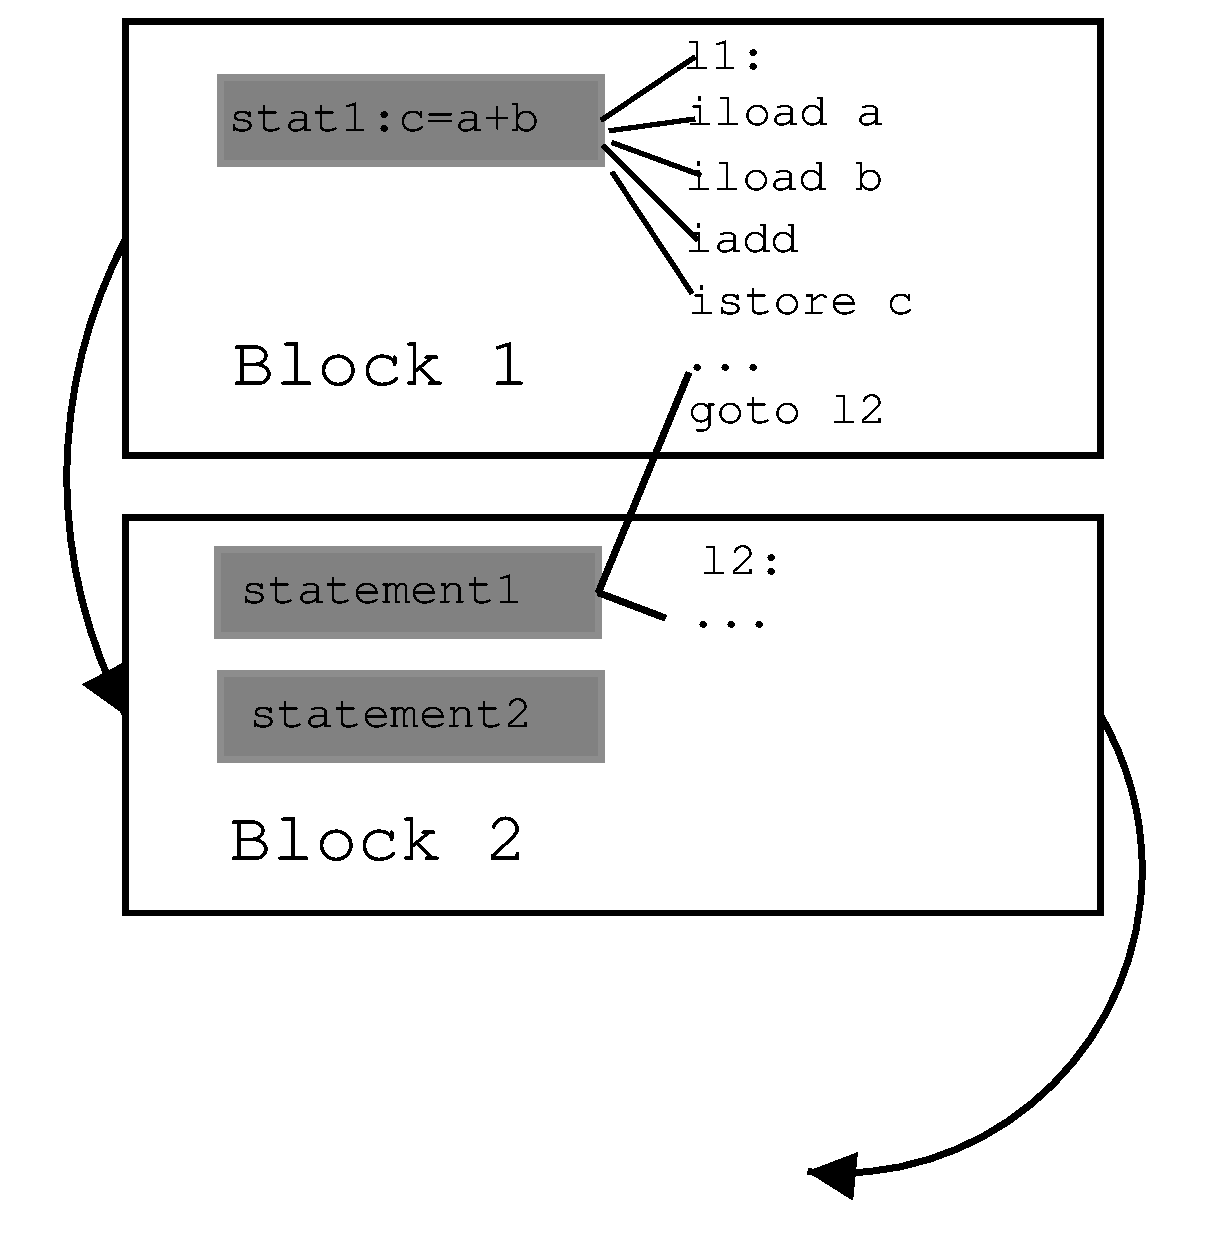
\includegraphics{cfg.eps}} \par}
\vspace{0.3cm}
Expression tree construction is also a tedious procedure.
BLOAT has a function to deal with the expression tree corresponding
to \textbf{every instruction}.  BLOAT also simulates the stack.
For one instuction, it pops the operands from the stack, then pushes
the expression of this instruction onto the stack and corresponding
edges are added between this expression and the operand expressions. If
this instruction does not represent an expression, nothing is pushed
onto the stack. Instead, an statement is generated which is actually
the root for the expression tree.  (The code is in Tree class)

The CFG traversal is a DFS (anti-DFS) traversal over blocks.
Inside a block, statements are traversed one by one.


\subsubsection{Dataflow analysis}

Given the complexity to build a pratical DF analyzer (the exception handler
code in particular frightens the authors), we don't
want to build a DF analyzer from scratch.  Most of the components
of a standard DF analyzer are already there. Blocks and edges between
them compose a conventional CFG which can be used to do dataflow
analysis.  The functions which deal with expression construction for
every instruction can be modified to do unit data flow procedure.
The simulated stack can be used to flow the data. Our solution follows from
these facts.

\begin{enumerate}
\item Divide the code list into blocks using the same method as CFG block division.
\item Add edges between blocks.  This is also part of the CFG building function.
At this point, we have a conventional CFG \emph{dcfg}(without the confusing expression
tree).
\item Generate a topological order for \emph{dcfg.} We have to get the
dominance to break a loop.
\item Traverse the blocks in a topological order. Store the range information
in the stack. Store 0 for iconst\_0, Store 1 for iconst\_1, Store the
current range of \emph{var} for \emph{iload var,} Store 0 for boolean
function. etc. The meet operation of the data flow is simply the union
of all the preceding stacks.
\item Finally, if a variable has {[}0,1{]} as its range, it is marked a
boolean variable. We also mark boolean array, Boolean, Boolean array.
\end{enumerate}
It turns out to be a nice solution to boolean local variable identification.
It considers those integer variable with range {[}0,1{]} as boolean.
But it doesn't matter.



\section{Splitting Techniques}
\begin{listing}{1}

public class Test {
    public static void main(String argv[]) {
	int i;
	boolean b,a[] = new boolean[16];
	b = false;
	for(i = 0 ; i < 16 ; i++) {
	    a[i] = b;
	    b = !b;
	}
	for(i = 0 ; i < 16 ; i++) {
	    System.out.println(a[i]);
	}
    }
}

\end{listing}

The boolean variable splitting techniques presented below will
be demonstrated on the sample code above.


\subsection{XOR Splitting}

The basic idea of the XOR splitting technique is as follows:

\begin{listing}{1}
	boolean a = true;
	boolean b = false;
\end{listing}

is converted to:

\begin{listing}{1}
	boolean a1 = true,a2 = false;
	boolean b1 = false,b2 = false;
\end{listing}

or

\begin{listing}{1}
	boolean a1 = false,a2 = true;
	boolean b1 = true,b2 = true;
\end{listing}

In general, a single boolean variable will be replaced with a pair of boolean
variables such that the state of the original variable at any program point
is equal to the XOR of the 2 new variables.  Likewise, a boolean array 'a' will 
be replaced by an array 'b' with twice as many elements, in which the state of
array element a[i] in the original array at any program point is equal to the XOR
of b[2*i] and b[2*i + 1].

\subsection{Parity Splitting}

The basic idea of parity splitting is to replace a single boolean variable
with a pair of integer variables that sum to an even number at every program
point where the original variable is false, and sum to an odd number otherwise.

\subsection{Equality Splitting}

The basic idea of equality splitting is to replace a boolean variable with a
pair of integer variables that have equal values at every program point where
the original variable is true, and unequal values otherwise.

\section{Code Transformation Techniques}

\subsection{Simple Variable Transformations}

Our implementation only obfuscates boolean variables where all assignments to
the variables are in one of the following forms:

\begin{listing}{1}
iconst_0
istore_1

<or>

iconst_1
istore_1
\end{listing}

or

\begin{listing}{1}
<compute integer condition>
ifeq L1
iconst_1
goto L2
L1:
iconst_0
L2:
istore_1
\end{listing}

These patterns are easily modified to work as split variables:

\begin{listing}{1}
ifeq L1
iconst_0
iconst_1
goto L2
L1:
iconst_1
iconst_1
L2:
istore_1
istore_2
\end{listing}

\subsection{Boolean Array Splitting Techniques}

Our implementation only obfuscates arrays that are allocated in a function and
used in specific ways exclusively in that function.  Allocation must look like this 
(all examples use the XOR obfuscation):

\begin{listing}{1}
newarray boolean
astore_1
\end{listing}

This pattern is converted to this pattern in the obfuscated code,
which produces an array that is twice as long:

\begin{listing}{1}
iconst_1
ishl
newarray boolean
astore_1
\end{listing}

All stores must look approximately like this:

\begin{listing}{1}
aload_1
iload_2
iload_2
ifeq L1
iconst_1
goto L2
L1:
iconst_0
L2:
bastore
\end{listing}

This pattern is obfuscated as follows:

\begin{listing}{1}
aload_1
iload_2
iconst_1
ishl
dup2
iload_3
ifeq L1
iconst_1
dup_x2
pop
iconst_0
goto L2
L1:
iconst_0
dup_x2
pop
iconst_0
L2:
bastore
bastore
\end{listing}

All uses must look approximately like this:

\begin{listing}{1}
aload_1
iload_2
baload
\end{listing}

This pattern is obfuscated as follows:

\begin{listing}{1}
aload_1
iload_2
iconst_1
ishl
dup
iconst_1
iadd
aload_1
swap
baload
dup_x2
pop
baload
ixor
\end{listing}
